\hypertarget{des-kangourous-mais-pas-que}{%
\section{Des kangourous, mais pas que
!}\label{des-kangourous-mais-pas-que}}

\emph{Jeudi 02 août 2018}

Dès le premier jour, ce qui nous a le plus marqué en Australie, c'est
les oiseaux. On les entend chanter du soir au matin, où que ce soit y
compris au cœur des grandes villes. Les petits loriquets viennent
réclamer du pain sur la terrasse le matin, le kookabura fait office de
réveil aux aurores avec son chant qui ressemble à un rire moqueur, les
cacatoès font un boucan d'enfer dans les parcs, les mouettes restent
fidèles à elles-mêmes et tournent autour des terrasses de \emph{fish and
chips} et les ibis font les poubelles avec leur long bec... On a aussi
croisé des pies dont le cri ressemble à R2-D2, des dindons sauvages dans
les forêts, de beaux perroquets à Kennett River, et même une chouette en
plein centre de Sydney !

Pour ce qui est des animaux terrestres, les incontournables kangourous
et leurs petits frères les wallabies se sont avérés très curieux, et les
koalas nous ont attendri, une fois qu'on a réussi à les voir !

\begin{figure}
\centering
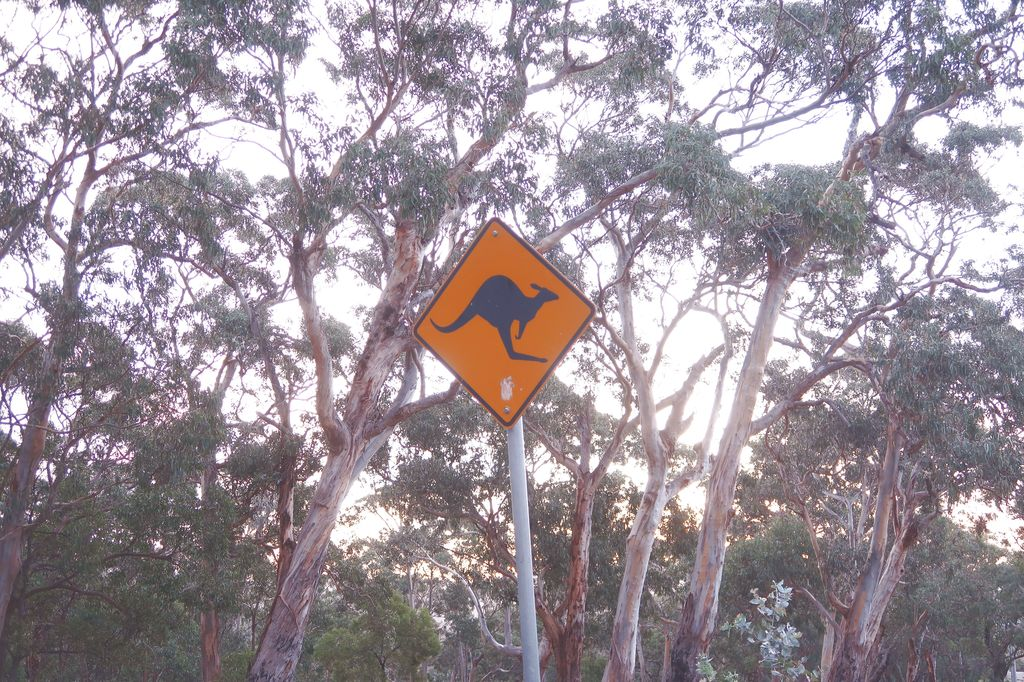
\includegraphics{images/20180802_kangourou.JPG}
\caption{Attention aux kangourous.}
\end{figure}

Comme les images valent mieux que mille mots, voici un condensé de ces
magnifiques animaux. On n'a pas réussi à trouver le nom de tous ces
animaux (surtout les oiseaux...), alors pour les ornithologues parmi
vous, n'hésitez pas à nous instruire :)

\emph{Elida et Florian}

\hypertarget{commentaires}{%
\subsection{Commentaires}\label{commentaires}}

\begin{itemize}
\item
  Franck Mazas, \emph{2018-08-14 10h47}

  Emu, en bon français, c'est plutôt émeu. Mettons ça sur le compte de
  l'émotion !\\
  Je suggérerais bien le développement d'un script Python pour la
  reconnaissance automatique des volatiles à partir d'une base de
  données, mais j'aurais trop peur que les pythons bouffent les oiseaux,
  c'est bien connu.
\item
  Florian LB, \emph{2018-08-16 07h39}

  Aaaah c'est pour ce genre de précision qu'on apprécie tes commentaires
  Franck ! Merci, je vais essayer de corriger ça. Quant au script
  python, il va devoir attendre je suis encore en vacances pour 3 mois
  :)
\item
  Didier VEZINET, \emph{2018-08-29 20h17}

  Le truc ou tu sêches c'est pas une variété de héron ?\\
  Ils sont trop mignons les wallabies :-)
\item
  Florian LB, \emph{2018-09-02 00h07}

  Des hérons... possible !\\
  C'est sûr que les wallabies et les kangourous, on les aurait bien
  approchés de plus près. Mais ils sont trop timides !
\end{itemize}
